\exercise{Basics}
Answer the following questions:
\begin{enumerate}
    \item In general, we can distinguish between two forms of machine learning.
    Which are these and how can we characterize them?
    \item Which traditional forms of machine learning do you know?
    \item Define the following terms:
    Hyperparameter, Bias, Classifier, Dataset, Clustering, Loss-Function, Class, Parameter, Datapoint, Variance, Regression, Training
\end{enumerate}
%
%
\exercise{Traditional Machine Learning Procedures}
Familiarize yourself with the provided script \mintinline{bash}{polynomial_fit.ipynb}.
Discuss strengths and weaknesses of the methods shown.
%
%
\section*{Understanding Neural Networks}
Let $\vec{x}=(x_1,\dots,x_n)$ be the input vector und $\vec{g}(\vec{x})=(\vec{g}(\vec{x})_1,\dots,\vec{g}(\vec{x})_m)$ the output vector of a neural network.
We denote the loss function (Cost-Funktion) with $C$ and with $L$ the number of layers.
The weights between layer $l-1$ and $l$ and between node $j$ of layer $l$ and node $k$ of layer $l-1$ are written as $W^l=w^l_{jk}$.
The number of nodes per layer $l$ is given by $\sigma_l$.
Figure~\ref{neural-network} shows an example for such a neural network.
\begin{figure}[htp]
    \centering
    \tikzset{%
        every neuron/.style={
            circle,
            draw,
            minimum size=1cm
        },
        neuron missing/.style={
            draw=none, 
            scale=3,
            text height=0.333cm,
            execute at begin node=\color{black}$\vdots$
        },
    }
    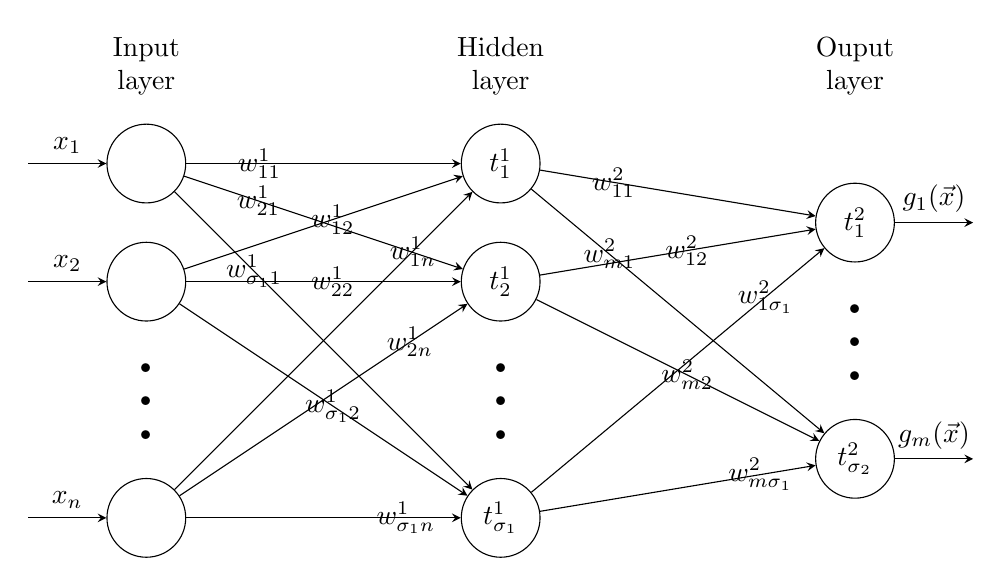
\begin{tikzpicture}[x=1.5cm, y=1.5cm, >=stealth]

        \foreach \m/\l [count=\y] in {1,2,missing,3}
        \node [every neuron/.try, neuron \m/.try] (input-\m) at (0,2-\y) {};

        \foreach \m [count=\y] in {1,2,missing,3}
        \node [every neuron/.try, neuron \m/.try ] (hidden-\m) at (3,2-\y) {\ifnum\y=3\else \ifnum\y=4 $t^1_{\sigma_1}$\else$t^1_{\m}$\fi\fi};

        \foreach \m [count=\y] in {1,missing,2}
        \node [every neuron/.try, neuron \m/.try ] (output-\m) at (6,1.5-\y) {\ifnum\y=2\else \ifnum\y=3 $t^2_{\sigma_2}$\else$t^2_{\m}$\fi\fi};

        \foreach \l [count=\i] in {1,2,n}
        \draw [<-] (input-\i) -- ++(-1,0)
            node [above, midway] {$x_\l$};

        \foreach \l [count=\i] in {1,m}
        \draw [->] (output-\i) -- ++(1,0)
            node [above, midway] {$g_\l(\vec{x})$};

        \foreach \i [count=\l] in {1,2,n}
        \foreach \j [count=\k] in {1,2,\sigma_1}
            \draw [->] (input-\l) -- (hidden-\k)
                node [pos=0.8*\l/3] {$w^1_{\j\i}$};
        
        \foreach \i [count=\l] in {1,2,\sigma_1}
        \foreach \j [count=\k] in {1,m}
            \draw [->] (hidden-\l) -- (output-\k)
                node [pos=0.8*\l/3] {$w^2_{\j\i}$};

        \foreach \l [count=\x from 0] in {Input, Hidden, Ouput}
        \node [align=center, above] at (\x*3,1.5) {\l \\ layer};
    \end{tikzpicture}
    \caption{Example of a neural network with only one hidden layer.}
    \label{neural-network}
\end{figure}
The total function $g$ of the layer can be split along the function of the individual layers $f^l$.
We can thus write
\begin{equation}
    \vec{g}(\vec{x}) = \vec{f}^L(W^L\vec{f}^{L-1}(W^{L-1}\dots \vec{f}^1(W^1\vec{x})\dots))
    \label{apply-layer-chain}
\end{equation}
We inspect the first layer of our example in figure~\ref{neural-network}.
Here, the result at the first hidden layer will be
\begin{align}
    t^1_j &= f^1\left(w^1_{j1}x_1 + w^1_{j2}x_2 + \dots + w^1_{jn}x_n\right)\\
    t^1_j &= f^1\left(\sum\limits_{k=0}^n w^1_{jk}x_k\right)
\end{align}
or generally speaking for a larger neural network
\begin{equation}
    t^{l+1}_j = f^{l+1}\left(\sum\limits_{k=0}^{\sigma_{l}} w^{l+1}_{jk} t^{l}_k\right).
\end{equation}
\exercise{Building Neural Networks}
\begin{enumerate}
    \item Build a neural network with one input node and one output node and no hidden layers.
    This network should return double its input value.
    Assume $f(x)=x$.
    How do we need to chose the weights?
    \item Extend the previous example to a vector, such that the result is of the same size buth with entries doubled.
    \item Build a neural network with no hidden layers and an input vector $(x_1,\dots,x_n)$ that puts out the sum of all entries of this vector.
    Still assume that $f(x)=x$.
    \item Build a neural network with no hidden layer that outputs the scalar product of two input vectors $v=(v_1,\dots,v_n)$ and $w=(w_1,\dots,w_n)$.
    Assume that all weights are exactly unity $w^l_{jk}=1$.
    How does the output layer look like?
    How do we need to choose $f$?
    \item Build a neural network that 
\end{enumerate}
%
%
\exercise{Backpropagation}
Backpropagation computes the gradient
\begin{equation}
    \frac{\partial C}{\partial w^l_{jk}}(\vec{g}(\vec{x}),\vec{y}) = \frac{\partial\vec{g}}{\partial w^l_{jk}}(\vec{x})\cdot\vec{\nabla}_yC\left(\vec{g}(\vec{x}), \vec{y}\right)
\end{equation}
at fixed input $\vec{x}$ and desired output $\vec{y}$ but with varying weights $w^l_{jk}$.
We could calculate this derivative by applying the chain rule iteratively to equation~\ref{apply-layer-chain} but this would be extremely inefficient.\\
Given a function
\begin{equation}
    G(x) = a(b(c(\dots z(x)\dots)))
\end{equation}
calculate the derivative with respect to $x$.
How can we generalize this behaviour for the general case
\begin{equation}
    x^l = f^l(x^{l-1})
\end{equation}
where $l\in\{0,\dots,n\}$?
What happens if we assume $f^l(x)=A^l g(x)$ where $A$ is a matrix?